\begin{exercises} 

\item \label{Ez:9.3.1}  Let $\vv = \langle -2, 5 \rangle$ in $\R^2$, and let $\vy = \langle 0, 3, -2 \rangle$ in $\R^3$. 

    \ba
    	\item Is $\langle 2, -1 \rangle$ perpendicular to $\vv$?  Why or why not?
	\item Find a unit vector $\vu$ in $\R^2$ such that $\vu$ is perpendicular to $\vv$.  How many such vectors are there?
	\item Is $\langle 2, -1, -2 \rangle$ perpendicular to $\vy$?  Why or why not?
	\item Find a unit vector $\vw$ in $\R^3$ such that $\vw$ is perpendicular to $\vy$.  How many such vectors are there?
	\item Let $\vz  = \langle 2, 1, 0 \rangle$.  Find a unit vector $\vr$ in $\R^3$ such that $\vr$ is perpendicular to both $\vy$ and $\vz$.  How many such vectors are there?
    \ea

\begin{exerciseSolution}

    \ba
    \item Since $\langle 2, -1 \rangle \cdot \langle -2, 5 \rangle = -9$ is not zero, the vector  $\langle 2, -1 \rangle$ is not perpendicular to $\vv$. 
	\item First we find a vector perpendicular to $\vv$. By inspection one such vector is $\vw=\langle 5, 2 \rangle$ (note that $\langle 5, 2 \rangle \cdot \vv = 0$). Then $\vu = \frac{1}{|\vw|} \vw = \frac{1}{\sqrt{29}} \langle 5,2 \rangle$ is a unit vector that is perpendicular to $\vv$.  There are exactly two unit vectors in $\R^2$ that are perpendicular to $\vv$: $\vu$ and $-\vu$. 
	\item The dot product of $\langle 2, -1, -2 \rangle$ with $\vy$ is 1, so these two vectors are not perpendicular. 
	\item The vector $\vy = \langle 0 , 2, 3 \rangle$ is perpendicular and so the vector $\vw = \frac{1}{|\vy|} \vy = \frac{1}{\sqrt{13}} \langle 0, 2, 3 \rangle$ is a unit vector in $\R^3$ that is perpendicular to $\vy$.  We can rotate the vector $\vw$ around the vector $\vv$ to obtain infinitely many different unit vectors in $\R^3$ that are perpendicular to $\vv$. 
	\item For a vector $\vr = \langle a,b,c \rangle$ to be perpendicular to both $\vy$ and $\vz$, we must have $\vr \cdot \vy = 0$ and $\vr \cdot \vz = 0$. This gives us two equations $3b-2c=0$ and $2a+b=0$. Thus, $b = -2a$ and $-6a-2c = 0$. So $c = -3a$. Thus, any vector of the form $\langle a, -2a, -3a \rangle$ is perpendicular to both $\vy$ and $\vz$. These vectors are all scalar multiples of the vector $\langle 1, -2, -3 \rangle$ with magnitude $\sqrt{14}$, and so there are just two vectors in $\R^3$ that are perpendicular to both $\vy$ and $\vz$: $\vr = \frac{1}{\sqrt{14}} \langle 1, -2, -3 \rangle$ and $-\vr$.   
    \ea
    
\end{exerciseSolution}

\item \label{Ez:9.3.2}  Consider the triangle in $\R^3$ given by $P(3, 2, -1)$, $Q(1, -2, 4)$, and $R(4, 4, 0)$.  
%Let $\va = \langle 2, -1, 1 \rangle$ and $\vb = \langle 1, 1, 3 \rangle$.

	\ba
		\item Find the measure of each of the three angles in the triangle, accurate to $0.01$ degrees.
		\item Choose two sides of the triangle, and call the vectors that form the sides (emanating from a common point) $\va$ and $\vb$.
			\begin{enumerate}[i.]
			\item Compute $\proj_{\vb} \va$, and $\proj_{\perp \vb} \va$.
			\item Explain why $\proj_{\perp \vb} \va$ can be considered a height of triangle $PQR$.
			\item Find the area of the given triangle.   
			\end{enumerate}
	\ea

\begin{exerciseSolution}

    \ba
    \item To find the angle between the sides $\overline{PQ}$ and $\overline{PR}$, we first we find the vectors that make up those sides of the triangle:  $\overrightarrow{PQ} = \langle -2, -4, 5 \rangle$, $\overrightarrow{PR} = \langle 1,2,1 \rangle$. Then the angle between $\overline{PQ}$ and $\overline{PR}$ is 
\[\cos^{-1}\left( \frac{\overrightarrow{PQ} \cdot \overrightarrow{PR}}{|\overrightarrow{PQ}| |\overrightarrow{PR}|} \right) = \cos^{-1}\left( \frac{-5}{\sqrt{45}\sqrt{6}}\right) \approx 107.72^{\circ}.\]
To find the angle between the sides $\overline{RQ}$ and $\overline{RP}$, we first we find the vectors that make up those sides of the triangle:  $\overrightarrow{RQ} = \langle -3, -6, 4 \rangle$, $\overrightarrow{RP} = \langle -1,-2,-1 \rangle$. Then the angle between $\overline{RQ}$ and $\overline{RP}$ is 
\[\cos^{-1}\left( \frac{\overrightarrow{RQ} \cdot \overrightarrow{RP}}{|\overrightarrow{RQ}| |\overrightarrow{RP}|} \right) = \cos^{-1}\left( \frac{11}{\sqrt{61}\sqrt{6}}\right) \approx 54.90^{\circ}.\]
To find the angle between the sides $\overline{QR}$ and $\overline{QP}$, we first we find the vectors that make up those sides of the triangle:  $\overrightarrow{QR} = \langle 3, 6, -4 \rangle$, $\overrightarrow{QP} = \langle 2,4,-5 \rangle$. Then the angle between $\overline{QR}$ and $\overline{QP}$ is 
\[\cos^{-1}\left( \frac{\overrightarrow{QR} \cdot \overrightarrow{QP}}{|\overrightarrow{QR}| |\overrightarrow{QP}|} \right) = \cos^{-1}\left( \frac{50}{\sqrt{61}\sqrt{45}}\right) \approx 17.38^{\circ}.\]
Note that  $107.72^{\circ} + 54.90^{\circ} + 17.38^{\circ} = 180^{\circ}$ as expected. 

	\item Choose two sides of the triangle, and call the vectors that form the sides (emanating from a common point) $\va$ and $\vb$.
		\begin{enumerate}[i.]
		\item Let $\va = \overrightarrow{PQ} = \langle -2, -4, 5 \rangle$ and $\vb = \overrightarrow{PR} = \langle 1,2,1 \rangle$. Then
\begin{align*}
\proj_{\vb} \va &= \frac{\va \cdot \vb}{\vb \cdot \vb} \vb = \frac{-5}{6} \langle 1,2,1 \rangle \\
\proj_{\va} \vb &= \frac{\vb \cdot \va}{\va \cdot \va} \va = \frac{-5}{45} \langle -2,-4,5 \rangle.
\end{align*}

		\item The vector $\proj_{\perp \vb} \va$ can be viewed as the vector from the tip of $\vb = \overrightarrow{PR}$ onto the line determined by the vector $\va$. This will be an altitude (or height) of the triangle. 
		\item The area of the triangle is one half the base times the height. We can use $\proj_{\perp \vb} \va$ as the height and $\va$ as teh base, so the area of the triangle is
\[\frac{1}{2} |\va| |\proj_{\perp \vb} \va| = \frac{1}{2} \sqrt{45} \left(\frac{5}{6}\right) \sqrt{6}.\]

	\end{enumerate}
    \ea
    
\end{exerciseSolution}

\item \label{Ez:9.3.3}    Let $\vu$ and $\vv$ be vectors in $\R^5$ with $\vu \cdot \vv = -1$, $| \vu | = 2$, $| \vv | = 3$, and $\theta$ the angle between $\vu$ and $\vv$. Use the properties of the dot product to find each of the following.
    \ba
    \item $\vu \cdot 2\vv$

    \item $(\vu + \vv) \cdot \vv$

    \item $(2\vu+4\vv) \cdot (\vu - 7\vv)$
    
    \item $\vv \cdot \vv$
    
    \item $|\vu| |\vv| \cos(\theta)$
    
    \item $\theta$

    \ea

\begin{exerciseSolution}
    \ba
    \item We know that we can factor scalars from dot products, so
\[\vu \cdot 2\vv = 2 (\vu \cdot \vv) = 2(-1) = -2.\]

    \item We know that $\vv \cdot \vv = |\vv|^2 = 9$.
    
    \item The dot product distributes over vector addition, so 
\[(\vu + \vv) \cdot \vv = (\vu \cdot \vv) + (\vv \cdot \vv) = (-1) + |\vv|^2 = (-1) + 9 = 8.\]

    \item Combing the distributive property of the dot product over vector addition, the fact that we can factor scalars from dot products, and that the dot product is commutative we see that  
\begin{align*}
(2\vu+4\vv) \cdot (\vu - 7\vv) &= 2(\vu \cdot \vu) - 14(\vu \cdot \vv) + 4(\vv \cdot \vu) - 28 (\vv \cdot \vv) \\
	&= 2(\vu \cdot \vu) - 14(\vu \cdot \vv) + 4(\vu \cdot \vv) - 28 (\vv \cdot \vv) \\
    &= 2(\vu \cdot \vu) - 10(\vu \cdot \vv) + 4(\vu \cdot \vv) \\
    &= 2|\vu|^2 - 10(\vu \cdot \vv) - 28 |\vv|^2 \\
    &= 8+10-252 \\
    &=-234.
 \end{align*}
 
    
    \item Given that $\cos(\theta) = \frac{\vu \cdot \vv}{|\vu| |\vv|}$, we have 
\[|\vu| |\vv| \cos(\theta) = \vu \cdot \vv = -1.\]
    
    \item In this case we have 
\[\theta = \cos^{-1}\left(\frac{\vu \cdot \vv}{|\vu| |\vv|}\right) = \cos^{-1}\left(\frac{-1}{6}\right) \approx 99.59^{\circ}.\] 

    \ea
    
\end{exerciseSolution}



%\item \label{Ez:9.3.1}   

%A tetrahedron is a four-sided solid in $\R^3$, each of whose faces are triangles.  Consider the tetrahedron whose vertices are the points $(1,0,0)$, $(0,1,0)$, $(1,0,0)$, and $(1,1,1)$ as shown in Figure
%\begin{figure}[ht]
%\begin{center}
 %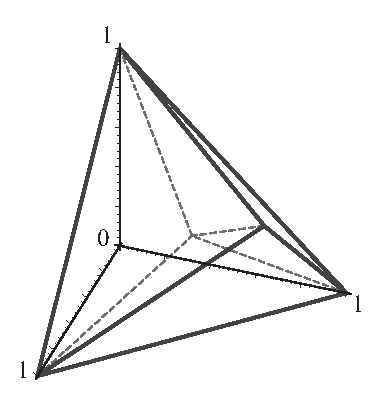
\includegraphics{figures/9_3_Ez1_tetrahedron.eps}
% \caption{The tetrahedron with vertices $(1,0,0)$, $(0,1,0)$, $(1,0,0)$, and $(1,1,1)$.} \label{F:9_3_Ez1_tetrahedron}
%\end{center}
%\end{figure}
%The \emph{centroid} of the tetrahedron is the average of the four vertices, which is the point $(\frac{1}{2}, \frac{1}{2}, \frac{1}{2})$, as shown at the intersection of the dotted lines.
 %   \ba
  %  	\item Consider the face determined by $(1,0,0)$, $(1,1,1)$, and $(0,0,1)$.  Explain why this face is an equilateral triangle.
%	\item 
 %   \ea

%\begin{exerciseSolution}
%\end{exerciseSolution}

\end{exercises}
\afterexercises
